% !TeX spellcheck = en_GB

\section{Problem 4}

We are monitoring a graph, which arrives as a stream of edges $\mathcal{E} = e_1, e_2, \ldots$. We
assume that exactly one edge arrives at a time, with edge $e_{i}$ arriving at time $i$, and the stream is starting at time 1. Each edge $e_{i}$ is a pair of vertices $(u_{i},v_{i})$, and we use $V$ to denote the set of all vertices that we have seen so far.\\
We assume that we are working in the sliding window model. According to that model, at each
time $t$ only the $w$ most recent edges are considered active. Thus, the set of active edges $E(t,w)$ at time $t$ and for window length $w$ is:
\begin{align*}
E(t,w) = 
	\left\{ \begin{aligned}
		&e_{t-w+1},\ldots,e_t &\quad\text{if }t > w\\
		&e_1,\ldots,e_t &\quad\text{if }t \le  w
	\end{aligned}\right.
\end{align*}
We then write $G(t,w) = (V,E(t,w))$ to denote the graph that consists of the active edges at time $t$, given a window length $w$.\\
As an example, given the stream of edges:
\begin{align*}
	e1 = (c,e), e2 = (b,d), e3 = (a,c), e4 = (c,b), e5 = (a,b), e6 = (c,d), e7 = (d,e)
\end{align*}
the graphs $G(5,5)$, $G(6,5)$ and $G(7,5)$ are shown below:
\begin{center}
	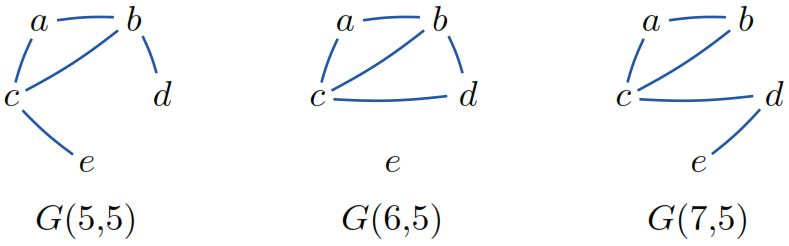
\includegraphics[scale=0.5]{img/example_graphs.jpg}
\end{center}
Notice that for all $t \ge w$ the graph $G(t+1,w)$ results from $G(t,w)$ by adding one edge and deleting one edge.\\
We want to monitor the connectivity of the graph $G(t,w)$. In other words, we want to design an
algorithm that quickly decides, at any time $t$, if the graph $G(t,w)$ is connected. In the previous example, the graphs $G(5,5)$ and $G(7,5)$ are connected, while the graph $G(6,5)$ is not connected.
\begin{enumerate}
	\item Propose a streaming algorithm for deciding the connectivity of $G(t,w)$.\\
	\textbf{Hint:} An efficient streaming algorithm takes advantage of the fact that the graph $G(t+1,w)$ changes very little compared to $G(t,w)$. Therefore, our algorithm should be able to efficiently update the connectivity of $G(t + 1,w)$ when a new edge $e_{t+1}$ arrives at time $t + 1$, given that the connectivity of $G(t,w)$ has already been computed.
	\item How much space does your algorithm use? Try to design an algorithm that manages to use
	$\mathcal{O}(n)$ space, where $n = |V|$.
	\item What is the update time of your algorithm?\\
	\textbf{Hint for 2 and 3:} The space of your algorithm is the maximum amount of space used at
	any given moment. The update time is the time needed to compute the output at time $t+1$,
	given the state at time $t$ and the new edge $e_{t+1}$ that arrives at time $t + 1$. You should provide your answer using the $\mathcal{O}(\cdot)$ notation, written as a function of the window length $w$ and the number of vertices $n$.
\end{enumerate}

\subsection{Streaming connectivity checking}

A \textbf{naive} solution for this problem would be performing a visit of the graph (DFS or BFS) each time the window slides forward, to check its connectivity. However, this simple algorithm has a \textbf{space} complexity equal to $\mathcal{O}(w)$, since all the edges in the window have to be kept in memory to perform the check, and a time complexity that is $\mathcal{O}(|V| + w)$, thus making the approach unfeasible in these settings.\\
Our idea is based on the fact that graph connectivity can be checked looking only at a \textbf{spanning tree} of $G$. Let $ST(G)$ be a spanning tree of $G$, then
\begin{align*}
ST(G)\text{ is connected }\Leftrightarrow \ G\text{ is connected}
\end{align*}
In addition, in this case, we want to consider $ST(G)$ such that it is made of the \textit{\textbf{most recent} edges in the window}: this way when an edge actually present in this spanning tree expires, then it would surely indicate a loss of connectivity in the overall graph. \\
Note that \textbf{checking connectivity} on the $ST(G)$ (again through a simple BFS or DFS) has \textbf{space} complexity
\begin{align*}
\mathcal{O}(|V|)
\end{align*}
since a tree has a number of edges that is at most $|V| - 1$.\\
Clearly, we also need to take into account the \textbf{time} complexity of managing the spanning tree. Again, a naive approach could be to rebuild it each time the window slides forward, but this would cost $\mathcal{O}(w)$ (unfeasible). A smarter approach would be to \textbf{update} it whenever the window moves, with a cost equal to $\mathcal{O}(|V|)$. A simple algorithm to do that is
\begin{enumerate}
	\item Add newly read edge to $ST(G)$.
	\item Detect the \textbf{loop} possibly introduced in step 1 (through a DFS much like we did in \textbf{Algorithm \ref{loop_check}}) and \textbf{delete the oldest edge} in it.
\end{enumerate}
Note that, since the graph trivially has \textbf{only one} loop, we have that $|V| = |E|$. Hence, \textbf{time} complexity of \textbf{Algorithm \ref{loop_check}} (in this case), and thus of our \textbf{update algorithm}, is
\begin{align*}
\mathcal{O}(|V|)
\end{align*}
What follows is the pseudocode of our streaming algorithm to decide whether $G(t,w)$ is connected.

\newpage
\setcounter{algorithm}{0}
\begin{algorithm}
	\caption{Check $G(t,w)$ connectivity}
	\begin{algorithmic}[1]
		\State $w \ \leftarrow \ \text{window size}$
		\State $st \ \leftarrow \ \text{empty spanning tree}$
		\Event{new edge $e_t = \langle u, v \rangle$ in stream}
			\State $st.addEdge(\langle u, v \rangle, \ t)$
			\State $st.removeCycle()$ \Comment delete oldest involved edge in (possible) cycle
            \State $st.removeEdge(t-w)$ \Comment delete (if present) edge with timestamp $t-w$
			\State \Return $st.isConnected()$  \Comment perform a BFS/DFS to check the connectivity
		\EndEvent
	\end{algorithmic}
\end{algorithm}
